%---------------------导言区---------------------------%
\documentclass[12pt,a4paper,UTF8]{ctexart}
	%10pt:正文字体为12pt,缺省为10pt;各层级字体大小会根据正文字体自动调整
	%a4paper:纸张大小a4;
	%UTF8:中文要求
%\usepackage{syntonly}
%\syntaxonly%加快编译速度
\usepackage{geometry}%用于设置上下左右页边距
	\geometry{left=2.5cm,right=2.5cm,top=3.2cm,bottom=2.8cm}
\usepackage{xeCJK,amsmath,paralist,enumerate,booktabs,multirow,graphicx,float,subfig,setspace,listings,lastpage,hyperref,gensymb}
	%xeCJK:中文字体(如楷体,作者和机构需要用到)的设置
	%amsmath:数学公式
	%paralist,enumerate:自定义项目符号
	%booktabs:三线图,论文常用的表格风格
	%multirow:复杂表格
	%graphicx,float: 插入图片
	%subfig:并排排版图片以及强制图表显示在“这里”[H]
	%setspace:设置行间距等功能
	\setlength{\parindent}{2em}%正文首行缩进两个汉字
	%listings:用于排版各种代码;比如matlab的代码
	%\lstset{language=Matlab}%matlab代码
	%lastpage:获取总页数;
	%hyperref:超链接,和lastpage搭配.
\usepackage{fancyhdr}
	%fancyhdr:一个很强大的宏包,用于自定义设计页面风格并命名以供调用。
	\pagestyle{fancy}
	\rhead{实验九~刚体转动实验}
	\lhead{普通物理实验\uppercase\expandafter{\romannumeral1}实验报告}
	\cfoot{\thepage}  
		%分别是右页眉、左页眉、右页脚
	\renewcommand{\headrulewidth}{0.4pt}
	\renewcommand{\theenumi}{(\arabic{enumi})}

\setCJKmainfont{FZSSK.TTF}[ItalicFont=FZKTK.TTF, BoldFont=FZHTK.TTF]
%中文字体设置:使用开源字体方正书宋,方正楷体和方正黑体



%%%%%%%%%%%%%%%%%%%%%%%%%%%%%%%%%%%%%%%%%%%%%%%%%%%%%%%%%%
%%%%%%%%%%%%%%%%%%%%%%%%%正文开始%%%%%%%%%%%%%%%%%%%%%%%%%%
%%%%%%%%%%%%%%%%%%%%%%%%%%%%%%%%%%%%%%%%%%%%%%%%%%%%%%%%%%

\begin{document}

%%begin-------------------标题与信息-----------------------%%

%%标题
\begin{center}
\LARGE\textbf{实验九~刚体转动实验}
\end{center}

%%信息
\begin{doublespacing}
	%doublespacing:手动两倍行距
	\centering
	\begin{tabular}{ll}
	 & \\
	{\CJKfontspec{STKAITI.TTF} 实验人:钟易轩}  & {\CJKfontspec{STKAITI.TTF}指导教师:王晨旭}\\
	{\CJKfontspec{STKAITI.TTF} 组号:九组七号} & {\CJKfontspec{STKAITI.TTF}学号:2000012706}\\
	{\CJKfontspec{STKAITI.TTF} 实验时间:2021年12月10日} &{\CJKfontspec{STKAITI.TTF} 实验地点:物理楼南楼~133}
	\end{tabular}
\end{doublespacing}

%%end-------------------标题与信息-----------------------%%

\subsection*{【实验目的】}
	\begin{enumerate}[(1)]
		\item 用转动法测定刚体转动惯量;
		\item 观测刚体的转动惯量随其质量和质量分布不同而改变的状况.
	\end{enumerate}
	
\subsection*{【仪器用具】}
	刚体转动实验装置,停表,砝码及砝码托,游标卡尺,钢卷尺等.
\subsection*{【实验数据处理】}
\subsubsection*{1.$\mathbf{m-\dfrac{1}{t^2}}$关系}
将一切装置安装并调节好之后,选择$r=2.50cm$的塔轮,再将圆柱形重物放置在$(5,5^{\prime})$的位置上.将$m$从一固定高度由静止落下,下落距离为$h=85.85cm$.改变$m$,每次增加$5.00g$,用停表计时三次取平均,得出表1.
\begin{table}[htbp]
\centering
\caption{实验一数据表}
\scalebox{1.1}{
\begin{tabular}{ccccccccc}
\toprule
$m/g$&5.00&10.00&15.00&20.00&25.00&30.00&35.00&40.00 \\
\hline
$t_1/s$&17.72&11.75&9.34&7.94&7.19&6.50&6.10&5.68 \\
\hline
$t_2/s$&18.16&11.71&9.16&8.07&6.97&6.44&5.97&5.53 \\
\hline
$t_3/s$&17.03&11.88&9.40&8.03&7.28&6.56&5.94&5.53 \\
\hline
$\bar t/s$&17.64&11.78&9.30&8.01&7.15&6.50&6.00&5.58 \\
\hline
$\dfrac{1}{t^2}\cdot(10^{-3}s^{-2})$&3.21&7.21&11.56&15.59&19.56&23.67&27.77&32.12 \\
\bottomrule
\end{tabular}}
\end{table}
\par
由于$m$的误差更小,因此选用$m$做自变量,$\dfrac{1}{t^2}$做因变量进行直线拟合.得出如下图像,
\newpage
\begin{figure}[htbp]
		\centering
		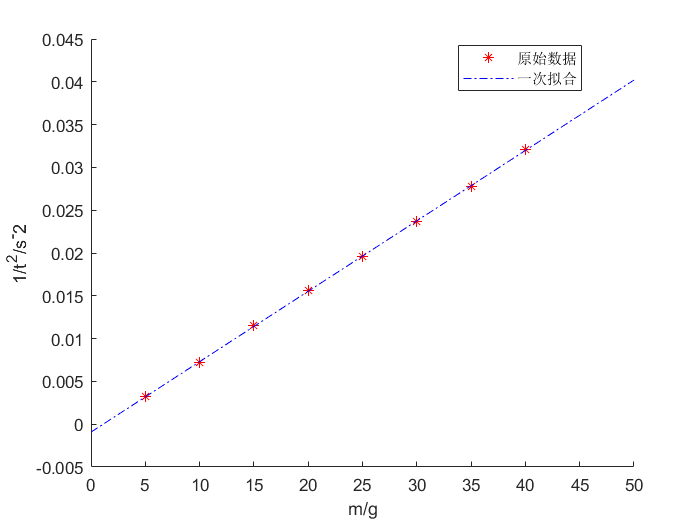
\includegraphics[width=9cm]{1.png}
		\caption{$m-\dfrac{1}{t^2}$线性回归图}
\end{figure}
\par
由方程$mgr-M_{\mu}=\dfrac{2hI}{rt^2}$得,有$\dfrac{1}{t^2}=\dfrac{gr^2}{2hI}m-\dfrac{M_{\mu}r}{2hI}$.通过回归计算得到$k=8.22548\times10^{-4}g^{-1}s^{-2}$,且有截距为$b=-9.21071\times10^{-4}s^{-2}$以及相关系数$r^2=0.99987$.则有$\dfrac{gr^2}{2hI}=8.22548\times10^{-4}$,又因为北京地区的重力加速度$g=9.81m/s^2$,因此可以求得$I=4.34(g\cdot m^2)$.\par
现在进行误差分析,由于$\sigma_k=\sqrt{\sigma_{k_{fit}}^2+\sigma_{k_y}^2+\sigma_{k_x}^2}$,其中有
\begin{align*}
	\sigma_{k_{fit}}&=k\sqrt{\frac{1/r^2-1}{8-2}}=3.83\times10^{-6} \\
	\sigma_{k_y}&=\frac{0.02}{\sqrt{3}\cdot t^3\cdot\sqrt{\sum_{i=1}^8(m_i-\bar m)^2}}=2.20\times10^{-6} \\
	\sigma_{k_x}&=k\frac{0.01}{\sqrt{3}\cdot \sqrt{\sum_{i=1}^8(m_i-\bar m)^2}}=3.88\times10^{-7}
\end{align*}
\par
又因为$I=\dfrac{gr^2}{2hk}$,则
\begin{equation*}
\sigma_I=\sqrt{(\frac{\partial I}{\partial r}\sigma_r)^2+(\frac{\partial I}{\partial h}\sigma_h)^2+(\frac{\partial I}{\partial k}\sigma_k)^2}
\end{equation*}
\par
由上述数据及公式可以得到$\sigma_I=0.0253(g\cdot m^2)$,则有$I=(4.34\pm0.03)g\cdot m^2$.
\subsubsection*{2.$\mathbf{r-\dfrac{1}{rt^2}}$关系}
保持$m=20.00g$不变,改变$r$的大小,重复之前的测量,得出表2.
\newpage
\begin{table}[htbp]
\centering
\caption{实验二数据表}
\scalebox{1.1}{
\begin{tabular}{cccccc}
\toprule
$r/cm$&0.991&1.510&2.003&2.500&2.999 \\
\hline
$t_1/s$&24.50&14.78&10.94&8.53&6.97 \\
\hline
$t_2/s$&24.29&14.69&10.84&8.37&7.09 \\
\hline
$t_3/s$&23.97&14.69&10.69&8.56&6.88 \\
\hline
$\bar t/s$&24.25&14.72&10.82&8.50&6.98 \\
\hline
$\dfrac{1}{rt^2}\cdot(10^{-3}cm^{-1}s^{-2})$&1.72&3.06&4.26&5.54&6.84 \\
\bottomrule
\end{tabular}}
\end{table}
\par
由于r的误差更小,因此将r作为自变量进行线性拟合,得出如下图像.
\begin{figure}[htbp]
		\centering
		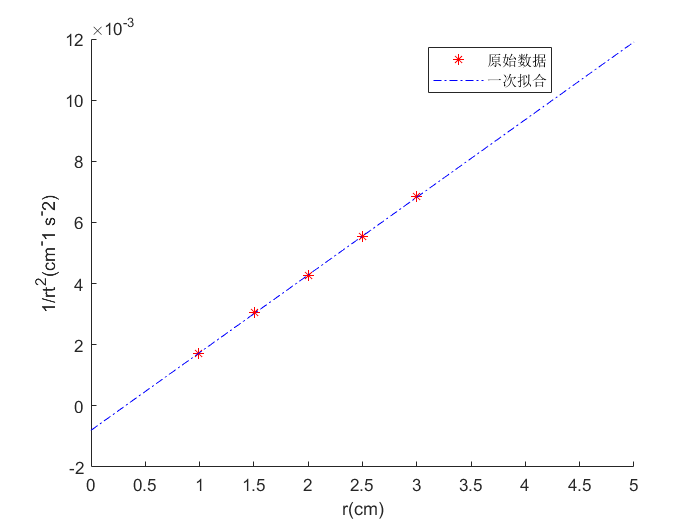
\includegraphics[width=9cm]{2.png}
		\caption{$r-\dfrac{1}{rt^2}$线性回归图}
\end{figure}
\par
由方程$mgr-M_{\mu}=\dfrac{2hI}{rt^2}$得,$\dfrac{1}{rt^2}=\dfrac{mg}{2hI}r-\dfrac{M_{\mu}}{2hI}$.\par
通过回归计算得到$k=0.00254(cm^{-2}\cdot s^{-2})$,$r^2=0.99984$.又由于$\dfrac{mg}{2hI}=k=0.00254$,则$I=4.49(g\cdot m^2)$.比第一个实验略大一点.现进行误差分析,由于$\sigma_k=\sqrt{\sigma_{k_{fit}}^2+\sigma_{k_y}^2+\sigma_{k_x}^2}$,其中有
\begin{align*}
	\sigma_{k_{fit}}&=k\sqrt{\frac{1/r^2-1}{5-2}}=1.86\times10^{-5}(cm^{-2}\cdot s^{-2}) \\
	\sigma_{k_y}&=\frac{3.11\times10^{-6}}{\sqrt{\sum_{i=1}^5(r_i-\bar r)^2}}=1.76\times10^{-6}(cm^{-2}\cdot s^{-2} )\\
	\sigma_{k_x}&=k\frac{1.15\times10^{-3}}{\sqrt{\sum_{i=1}^5(r_i-\bar r)^2}}=1.65\times10^{-6}(cm^{-2}\cdot s^{-2}) \\
\end{align*}
\par
因为$I=\dfrac{mg}{2hk}$,则有
\begin{equation*}
	\sigma_I=\sqrt{(\frac{\partial I}{\partial m}\sigma_m)^2+(\frac{\partial I}{\partial h}\sigma_h)^2+(\frac{\partial I}{\partial k}\sigma_k)^2}
\end{equation*}
\par
$\sigma_k=1.88\times10^{-5}(cm^{-2}\cdot s^{-2})$,代入上式中得到$\sigma_I=0.0057(g\cdot m^2)$,则有$I=(4.49\pm0.01)g\cdot m^2$.
\subsubsection*{3.转动惯量和质量分布的关系}
维持$m=10.00g$,以及$r=2.500cm$.对称地改变$m_0$的位置,得出表3.
\begin{table}[htbp]
\centering
\caption{实验三数据表}
\scalebox{1.1}{
\begin{tabular}{cccccc}
\toprule
&$(5,5^{\prime})$&$(4,4^{\prime})$&$(3,3^{\prime})$&$(2,2^{\prime})$&$(1,1^{\prime})$ \\
\hline
$x/cm$&13.315&10.800&8.287&5.781&3.450 \\
\hline
$t_1/s$&13.72&11.13&10.06&8.66&7.57 \\
\hline
$t_2/s$&13.37&11.25&10.18&8.75&7.62 \\
\hline
$t_3/s$&13.69&11.44&10.25&8.91&7.81 \\
\hline
$\bar t/s$&13.59&11.27&10.16&8.77&7.67 \\
\hline
$x^2/cm^2$&177.19&116.64&68.67&33.42&11.90 \\
\hline
$t^2/s^2$&184.69&127.01&103.23&76.91&58.83 \\
\bottomrule
\end{tabular}}
\end{table}
\par
经过线性拟合之后,得出如下图像,
\begin{figure}[htbp]
		\centering
		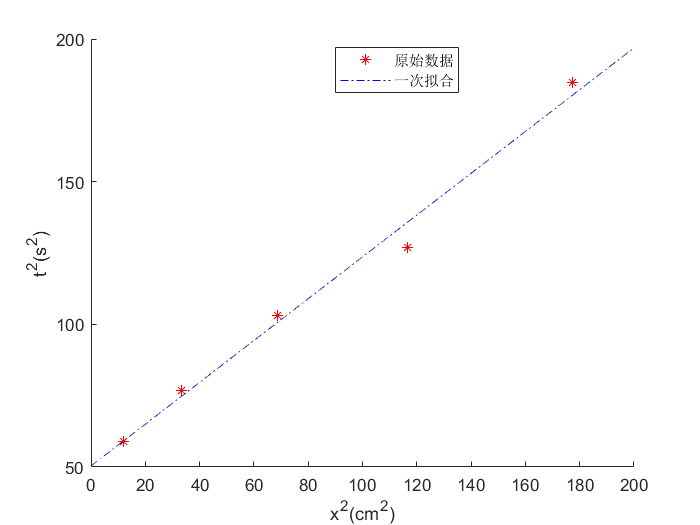
\includegraphics[width=9cm]{3.png}
		\caption{$t^2-x^2$线性回归图}
\end{figure}
\par
该拟合的相关因子为$r=0.9944$,说明直线拟合是较为成功的,因此$t^2$与$x^2$具有线性关系.
\subsection*{【分析与讨论】}
\subsubsection*{1.总结从调节实验装置和操作两个方面,怎样做才能减小在实验中产生的系统误差和随机误差?}
\textbf{(1)减小系统误差的方法:}\par
(a)在安装塔轮之前一定要调整架台垂直,并且安装塔轮时既要使其能转起来同时也要让其不能发生太强的晃动,以减小摩擦力矩变化的影响.\par
(b)绕线密绕,否则会造成摩擦力矩的改变.\par
(c)保持线垂直于桌沿,并且在改变r的时候也要改变滑轮的高度.\par
\textbf{(2)减小随机误差的方法:}\par
(a)多次测量求平均.\par
(b)最小二乘法线性拟合.\par
(c)注意秒表的掐表时刻,尽量保持在同一种时刻点.
\subsubsection*{2.【思考题(5)】用实验数据分析实验二中的I偏大的原因.}
在实验二中因为对r进行了改变,而在实验过程中发现当$r=0.991cm$以及$r=1.510cm$时不能够完全密绕,因此会导致$M_{\mu}$减小,因此会导致I增大.因此经过线性拟合之后,总体的I就变大了.
\subsection*{【收获与感想】}
不停地蹲起与缠线对体力是一个考验,因此对身体的锻炼还要加强;在做实验之前一定要把所有预备工作做好;用线性关系检查数据的正确性.












\end{document}
